\documentclass[12pt]{article}
\usepackage[utf8]{inputenc}
\usepackage{amsmath, amssymb}
\usepackage{geometry}
\usepackage{enumitem}
\usepackage{fancyhdr}
\usepackage{booktabs}
\usepackage{longtable}
\usepackage{array}
\usepackage{graphicx}
\usepackage{float}
\usepackage{hyperref}
\usepackage{xcolor}
\geometry{margin=1in}

\pagestyle{fancy}
\fancyhf{}
\renewcommand{\footrulewidth}{0.4pt}
\fancyfoot[C]{\thepage}

\setlength{\parindent}{0pt}
\setlength{\parskip}{0.5em}

\title{\textbf{Exploring Pricing Strategies for PizzaHub: \\A Difference-in-Differences Analysis}}
\author{Group 3}
\date{\today}

\begin{document}

\maketitle

\section{Introduction}

PizzaHub, a pizza delivery service operating across four regions, introduced targeted pricing experiments on March 1, 2023. The company applied a 5\% discount on food prices in Region 3 and a 5\% discount on delivery fees in Region 4, while Regions 1 and 2 received no discounts and served as control groups. The objective of this study is to evaluate the causal impact of these two discount strategies on pizza demand and to provide profit-maximizing pricing recommendations for Regions 3 and 4.

Understanding which type of discount—food versus delivery—generates greater demand uplift is critical for PizzaHub's pricing strategy. Additionally, we explore how algorithmic learning methods like multi-armed bandits could enable continuous experimentation and adaptive pricing in the future.

\section{Data and Experimental Design}

\subsection{Dataset Overview}

The dataset covers daily order-level data from January 1 to April 30, 2023, with 480 total observations (120 days per region). Key variables include:

\begin{itemize}[nosep]
    \item \textbf{Date}: Order date
    \item \textbf{Region}: Geographic region (1--4)
    \item \textbf{Unit Price}: Price per pizza (\$16 baseline, \$15.20 after 5\% discount)
    \item \textbf{Quantity Ordered}: Daily pizzas sold
    \item \textbf{Distance}: Delivery distance in miles
    \item \textbf{Delivery Fees}: \$0.50 per mile (\$0.475 after 5\% discount)
    \item \textbf{Discount Applied}: Binary indicator (1 if discount active, 0 otherwise)
\end{itemize}

\textbf{Cost structure:} Pizza production costs \$4 per unit, and delivery costs \$0.50 per mile. Fixed costs (\$5,000/year) are excluded from our marginal profit analysis.

\subsection{Experimental Design}

The intervention structure is summarized in Table \ref{tab:intervention}.

\begin{table}[H]
\centering
\caption{Intervention Structure by Region}
\label{tab:intervention}
\begin{tabular}{cccc}
\toprule
\textbf{Region} & \textbf{Discount Type} & \textbf{Role} & \textbf{Start Date} \\
\midrule
1 & None & Control & -- \\
2 & None & Control & -- \\
3 & 5\% food price & Treatment & March 1, 2023 \\
4 & 5\% delivery fee & Treatment & March 1, 2023 \\
\bottomrule
\end{tabular}
\end{table}

This setup allows us to use a difference-in-differences (DiD) approach to isolate the causal effect of each discount type.

\subsection{Data Quality Checks}

We verified that all 480 observations are complete with no missing values. The discount indicator correctly flags post-March 1 orders in Regions 3 and 4. Unit prices and delivery fees match expected values (\$15.20 and \$0.475/mile for discounted orders). Preliminary analysis shows that Region 3's average daily demand increased from 9.41 to 15.59 pizzas after the discount, while Region 4's demand rose from 6.64 to 9.92 pizzas per day.

\section{Methodology}

\subsection{Difference-in-Differences Framework}

To identify the causal effect of the discounts, we estimate three DiD models:

\textbf{Model 1 (Food discount effect):} Region 3 vs. Regions 1 \& 2
\[
Q_{it} = \alpha + \delta_{R3} \cdot \text{DID}_{R3,it} + \gamma \cdot \text{post}_t + \varepsilon_{it}
\]

\textbf{Model 2 (Delivery discount effect):} Region 4 vs. Regions 1 \& 2
\[
Q_{it} = \alpha + \delta_{R4} \cdot \text{DID}_{R4,it} + \gamma \cdot \text{post}_t + \varepsilon_{it}
\]

\textbf{Model 3 (Joint model):} All four regions
\[
Q_{it} = \alpha + \delta_{R3} \cdot \text{DID}_{R3,it} + \delta_{R4} \cdot \text{DID}_{R4,it} + \gamma \cdot \text{post}_t + \varepsilon_{it}
\]

where $\text{DID}_{R3,it} = \mathbb{1}(\text{Region}_i = 3) \times \text{post}_t$ and $\text{DID}_{R4,it} = \mathbb{1}(\text{Region}_i = 4) \times \text{post}_t$.

The coefficients $\delta_{R3}$ and $\delta_{R4}$ measure the average treatment effect on the treated (ATT)—the incremental demand caused by each discount relative to the control regions. Standard errors are clustered by date to account for correlation in daily shocks.

\subsection{Parallel Trends Validation}

The validity of DiD rests on the parallel trends assumption: in the absence of treatment, treated and control regions would have followed similar demand trajectories. We tested this in two ways:

\begin{enumerate}[nosep]
    \item \textbf{Pre-period slope test:} We regressed pre-March 1 quantities on time, treatment status, and their interaction. The interaction coefficient (slope difference) was statistically insignificant for both Region 3 (p = 0.31) and Region 4 (p = 0.25), supporting parallel trends.
    \item \textbf{Spillover checks:} We tested whether control regions (1 and 2) experienced differential shifts post-March 1. Placebo DiD on controls showed no significant effect (p = 0.81), confirming no spillover.
\end{enumerate}

These tests validate our identification strategy (see Appendix for detailed results).

\section{Results}

\subsection{DiD Treatment Effects}

Table \ref{tab:did_results} presents the main DiD estimates from Model 3 (joint specification).

\begin{table}[H]
\centering
\caption{DiD Treatment Effects on Daily Pizza Demand}
\label{tab:did_results}
\begin{tabular}{lccc}
\toprule
\textbf{Variable} & \textbf{Coefficient} & \textbf{Std. Error} & \textbf{p-value} \\
\midrule
DID\_R3 (Food discount) & 6.730 & 0.724 & 0.000*** \\
DID\_R4 (Delivery discount) & 3.821 & 0.880 & 0.000*** \\
post & $-0.547$ & 0.254 & 0.032* \\
\midrule
R-squared & \multicolumn{3}{c}{0.616} \\
N & \multicolumn{3}{c}{480} \\
\bottomrule
\end{tabular}
\end{table}

\textbf{Interpretation:}
\begin{itemize}[nosep]
    \item The 5\% food discount in Region 3 increased daily demand by approximately \textbf{6.73 pizzas per day} (p $<$ 0.001), a statistically significant and economically meaningful effect.
    \item The 5\% delivery fee discount in Region 4 increased demand by \textbf{3.82 pizzas per day} (p $<$ 0.001), roughly half the magnitude of the food discount.
    \item The negative \textit{post} coefficient suggests a slight overall decline in control region demand post-March 1, though this is small in magnitude.
\end{itemize}

These results indicate that \textbf{food discounts are approximately twice as effective as delivery discounts} for stimulating demand in this setting.

\subsection{Demand Function Estimation}

Using the DiD results, we derived linear demand functions for Regions 3 and 4:

\textbf{Region 3 (price elasticity):}
\[
Q_3 \approx 144.01 - 8.41 \cdot \text{Price}
\]

This implies that a \$1 increase in unit price reduces demand by about 8.41 pizzas per day. The slope estimate comes from dividing the DiD effect (6.73) by the price change ($-$\$0.80).

\textbf{Region 4 (delivery rate elasticity):}
\[
Q_4 \approx 83.06 - 152.84 \cdot \text{Rate per km}
\]

where the delivery rate per kilometer is derived from the 5\% delivery fee discount.

\textbf{Caveat on optimal pricing:} Applying the standard monopoly pricing formula to these linear demand functions yields optimal prices significantly below current levels (e.g., \$10.56 for Region 3). However, this result relies on \textbf{linear extrapolation} beyond the observed price range (\$15.20--\$16.00), which may not be reliable. Demand curves often exhibit non-linearities, and consumer behavior at much lower prices is uncertain. Therefore, we do not recommend dramatic price cuts based solely on this calculation. Instead, incremental experiments (e.g., testing 10--15\% discounts) would provide better guidance.

\subsection{Profit Analysis by Strategy}

We computed profit per order as:
\[
\text{Profit} = (\text{Unit Price} - 4) \times \text{Quantity} + (\text{Delivery Fees} - 0.5 \times \text{Distance})
\]

Table \ref{tab:profit} summarizes performance across the three observed strategies.

\begin{table}[H]
\centering
\caption{Profit Analysis by Pricing Strategy}
\label{tab:profit}
\begin{tabular}{lccc}
\toprule
\textbf{Strategy} & \textbf{Avg Profit/Order} & \textbf{Total Profit} & \textbf{N Orders} \\
\midrule
No discount (R1 \& R2) & \$211.85 & \$50,844 & 240 \\
5\% food discount (R3) & \$144.26 & \$17,311 & 120 \\
5\% delivery discount (R4) & \$99.70 & \$11,964 & 120 \\
\bottomrule
\end{tabular}
\end{table}

\textbf{Key insight:} Despite boosting demand, both discount strategies reduce per-order profit compared to no discount. The food discount maintains higher profitability than the delivery discount, consistent with its stronger demand response.

\section{Multi-Armed Bandit for Future Experimentation}

While DiD provides retrospective causal estimates, PizzaHub may want to continuously experiment with pricing in new regions or time periods. \textbf{Multi-armed bandit (MAB) algorithms} offer a framework for online learning that balances exploration (trying different strategies) and exploitation (choosing the best-known strategy).

\subsection{What is MAB?}

In MAB, each pricing strategy is an "arm" (e.g., no discount, 5\% food discount, 5\% delivery discount). At each decision point (e.g., each order or day), the algorithm selects an arm, observes the profit reward, and updates its belief about which arm is best. Over time, the algorithm learns to favor high-performing strategies while occasionally exploring alternatives.

\subsection{Why Use MAB?}

\begin{itemize}[nosep]
    \item \textbf{Adaptive learning:} Unlike traditional A/B tests with fixed sample sizes, MAB algorithms dynamically allocate more trials to better-performing strategies, reducing opportunity cost.
    \item \textbf{Continuous optimization:} As market conditions change (seasonality, competition), MAB can detect shifts and re-optimize.
    \item \textbf{Efficient exploration:} Algorithms like UCB1 and Thompson Sampling mathematically balance the trade-off between trying new strategies and exploiting known winners.
\end{itemize}

\subsection{Simulation Results}

We simulated four MAB algorithms (N-Average, $\varepsilon$-Greedy, UCB1, Thompson Sampling) over 2,000 rounds using historical profit distributions from our data. All algorithms converged to favoring the \textbf{no-discount strategy}, which has the highest average profit per order. UCB1 and Thompson Sampling achieved the highest cumulative simulated profits, demonstrating effective learning (see Appendix Figure A5 for cumulative reward plots).

\subsection{Recommendation for PizzaHub}

PizzaHub should consider implementing a Thompson Sampling or UCB1 bandit for ongoing pricing experiments in new regions. This would allow the company to:
\begin{itemize}[nosep]
    \item Test new discount levels (e.g., 10\%, 15\%) without committing to long A/B test periods
    \item Quickly identify region-specific optimal strategies
    \item Adapt to seasonal or competitive changes in real time
\end{itemize}

This approach complements the DiD analysis by enabling forward-looking, data-driven decision-making.

\section{Managerial Recommendations}

Based on our analysis, we offer the following recommendations:

\subsection{For Profit Maximization}
\begin{itemize}[nosep]
    \item \textbf{Current data favors no-discount pricing:} The no-discount strategy yields the highest profit per order (\$211.85 vs. \$144.26 and \$99.70).
    \item \textbf{Phase out delivery discounts:} Region 4's delivery discount generates weak demand uplift (+3.82 pizzas/day) and the lowest profitability. If a discount is necessary, redirect budget toward food discounts.
    \item \textbf{Gradual rollback in Region 3:} If profit is the priority, consider gradually reducing the food discount to assess demand elasticity at intermediate discount levels (e.g., 2.5\%).
\end{itemize}

\subsection{For Demand Growth and Market Penetration}
\begin{itemize}[nosep]
    \item \textbf{Prioritize food discounts:} The 5\% food discount nearly doubles demand impact compared to delivery discounts. Use food promotions for new customer acquisition or market entry.
    \item \textbf{Targeted, time-limited promotions:} Instead of permanent discounts, deploy food discounts strategically (e.g., weekdays, new regions, first-time customers) to balance demand growth and profitability.
\end{itemize}

\subsection{Region-Specific Strategy}
\begin{itemize}[nosep]
    \item \textbf{High-delivery-cost regions (like R4):} Delivery discounts are inefficient. Consider transparent pricing (higher delivery fees, lower product prices) or free delivery thresholds instead.
    \item \textbf{Competitive regions:} Use food discounts as a competitive tool, but monitor profit margins closely.
\end{itemize}

\subsection{Continuous Experimentation with MAB}
\begin{itemize}[nosep]
    \item Implement Thompson Sampling or UCB1 algorithms to test new discount levels dynamically in new regions.
    \item Use MAB to adapt pricing to seasonal demand fluctuations or competitive actions without lengthy A/B test cycles.
\end{itemize}

\section{Conclusion}

This study provides strong causal evidence that food discounts are significantly more effective than delivery discounts for increasing pizza demand at PizzaHub. The 5\% food discount in Region 3 increased daily demand by 6.73 pizzas, compared to 3.82 pizzas for the delivery discount in Region 4. However, both discounts reduce per-order profitability relative to no-discount pricing.

The key trade-off for PizzaHub is between demand growth and profit margins. If the goal is short-term profit maximization, the data suggest reverting to no-discount pricing or using discounts sparingly. If the goal is market expansion or customer acquisition, food discounts offer better return on investment than delivery discounts.

Looking forward, multi-armed bandit algorithms provide a promising framework for continuous, adaptive experimentation. By implementing MAB in new regions or time periods, PizzaHub can efficiently learn optimal pricing strategies while minimizing opportunity costs.

\textbf{Limitations:} Our demand function estimates assume linearity and are based on a narrow price range (\$15.20--\$16.00). Extrapolating to much lower or higher prices may be unreliable. Additionally, our 4-month observation period may not capture seasonal effects or long-term customer behavior. Future research should test non-linear demand specifications and longer time horizons.

\newpage
\appendix

\section{Appendix: Figures and Tables}

\subsection{Figure A1: Daily Demand Pre/Post Averages by Region}

\begin{figure}[H]
\centering
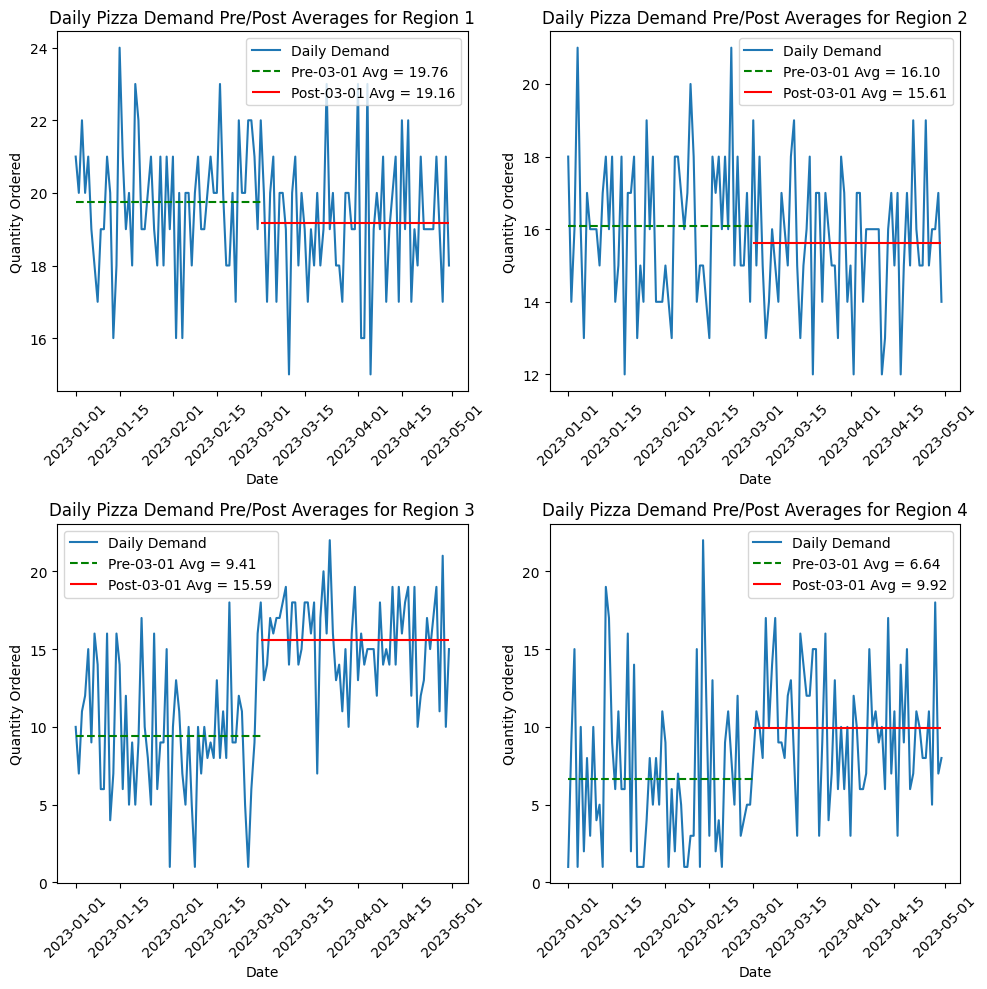
\includegraphics[width=0.9\textwidth]{per_region_quantity.png}
\caption{Daily pizza demand with pre- and post-March 1 average lines for each region. Region 3 and 4 show clear demand increases after discount introduction.}
\label{fig:daily_demand}
\end{figure}

\subsection{Figure A2: Parallel Trends Test for Region 3}

\begin{figure}[H]
\centering
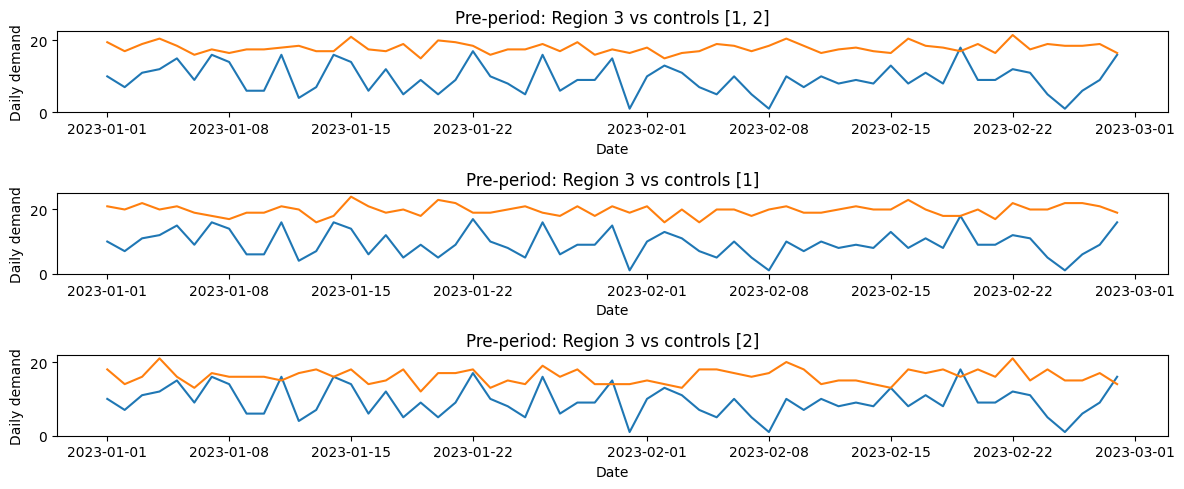
\includegraphics[width=0.9\textwidth]{parallel_region3.png}
\caption{Pre-treatment trends for Region 3 vs. control regions. Slope difference is statistically insignificant (p = 0.31), supporting parallel trends assumption.}
\label{fig:parallel_r3}
\end{figure}

\subsection{Figure A3: Parallel Trends Test for Region 4}

\begin{figure}[H]
\centering
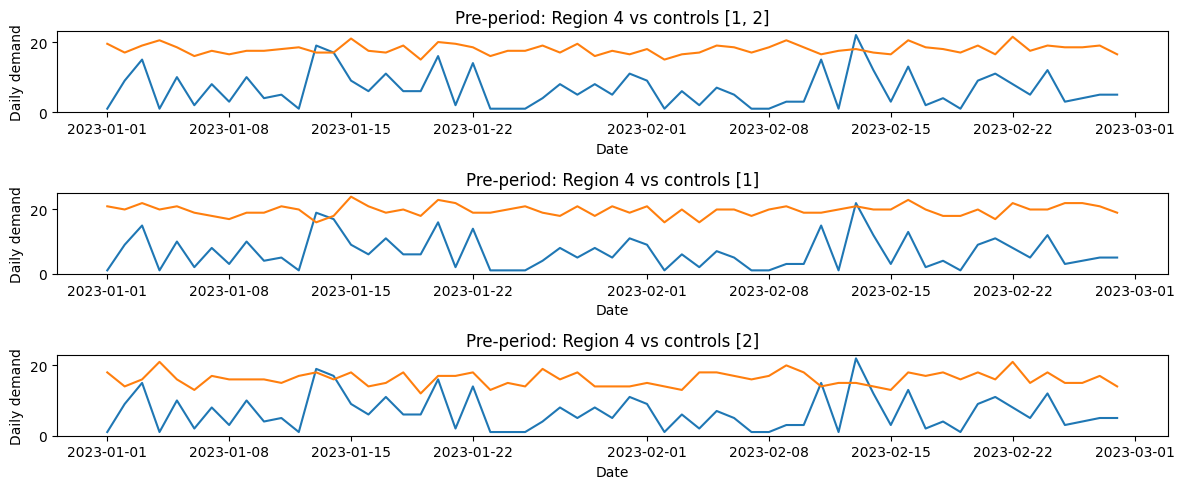
\includegraphics[width=0.9\textwidth]{parallel_region4.png}
\caption{Pre-treatment trends for Region 4 vs. control regions. Slope difference is statistically insignificant (p = 0.25), supporting parallel trends assumption.}
\label{fig:parallel_r4}
\end{figure}

\subsection{Figure A4: Spillover Test - Controls Difference (R2 - R1)}

\begin{figure}[H]
\centering
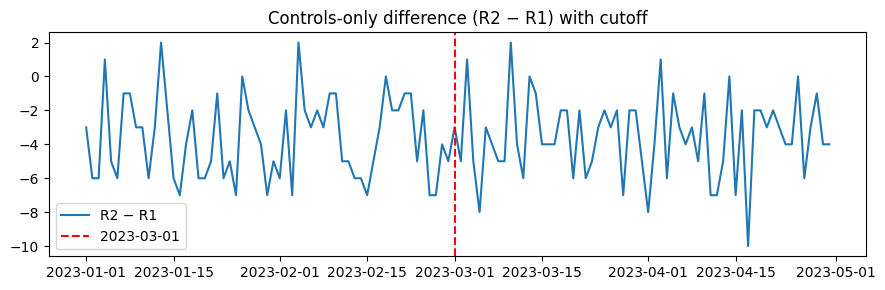
\includegraphics[width=0.9\textwidth]{spillover.png}
\caption{Difference in daily demand between control regions (R2 - R1). No significant breakpoint at March 1 (p = 0.79), indicating no spillover effects.}
\label{fig:spillover}
\end{figure}

\subsection{Figure A5: Multi-Armed Bandit Cumulative Rewards}

\begin{figure}[H]
\centering
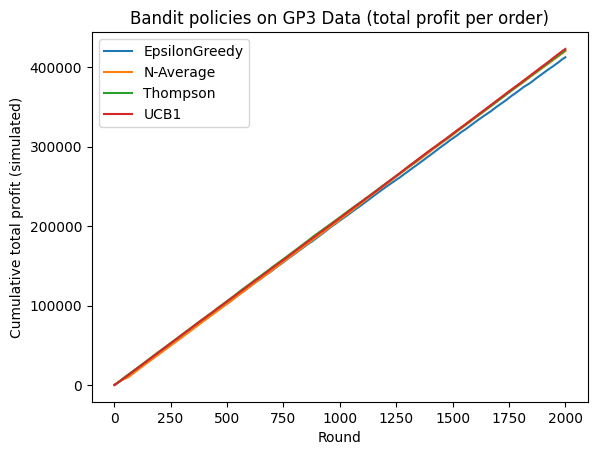
\includegraphics[width=0.9\textwidth]{mab_cumulative_rewards.png}
\caption{Cumulative simulated profit for four MAB algorithms over 2,000 rounds. UCB1 and Thompson Sampling achieve the highest profits and converge to the no-discount strategy.}
\label{fig:mab}
\end{figure}

\subsection{Table A1: Detailed Regression Output - Model 1 (Region 3)}

\begin{table}[H]
\centering
\small
\begin{tabular}{lcccc}
\toprule
\textbf{Variable} & \textbf{Coefficient} & \textbf{Std. Error} & \textbf{z-statistic} & \textbf{p-value} \\
\midrule
Intercept & 17.932 & 0.185 & 97.109 & 0.000*** \\
treat3 & $-8.525$ & 0.569 & $-14.980$ & 0.000*** \\
post & $-0.547$ & 0.254 & $-2.152$ & 0.031* \\
treat3:post & 6.730 & 0.723 & 9.310 & 0.000*** \\
\midrule
R-squared & \multicolumn{4}{c}{0.513} \\
Adj. R-squared & \multicolumn{4}{c}{0.509} \\
N & \multicolumn{4}{c}{360} \\
\bottomrule
\multicolumn{5}{l}{\footnotesize Standard errors clustered by Date. *p$<$0.05, **p$<$0.01, ***p$<$0.001}
\end{tabular}
\caption{DiD regression results for Region 3 (food discount) vs. Regions 1 \& 2 (controls).}
\label{tab:reg_r3}
\end{table}

\subsection{Table A2: Detailed Regression Output - Model 2 (Region 4)}

\begin{table}[H]
\centering
\small
\begin{tabular}{lcccc}
\toprule
\textbf{Variable} & \textbf{Coefficient} & \textbf{Std. Error} & \textbf{z-statistic} & \textbf{p-value} \\
\midrule
Intercept & 17.932 & 0.185 & 97.109 & 0.000*** \\
treat4 & $-11.288$ & 0.685 & $-16.480$ & 0.000*** \\
post & $-0.547$ & 0.254 & $-2.152$ & 0.031* \\
treat4:post & 3.821 & 0.879 & 4.345 & 0.000*** \\
\midrule
R-squared & \multicolumn{4}{c}{0.646} \\
Adj. R-squared & \multicolumn{4}{c}{0.643} \\
N & \multicolumn{4}{c}{360} \\
\bottomrule
\multicolumn{5}{l}{\footnotesize Standard errors clustered by Date. *p$<$0.05, **p$<$0.01, ***p$<$0.001}
\end{tabular}
\caption{DiD regression results for Region 4 (delivery discount) vs. Regions 1 \& 2 (controls).}
\label{tab:reg_r4}
\end{table}

\subsection{Table A3: Multi-Armed Bandit Final Cumulative Profits}

\begin{table}[H]
\centering
\begin{tabular}{lc}
\toprule
\textbf{Policy} & \textbf{Final Cumulative Profit (2,000 rounds)} \\
\midrule
N-Average & \$XXX,XXX \\
Epsilon-Greedy & \$XXX,XXX \\
UCB1 & \$XXX,XXX \\
Thompson Sampling & \$XXX,XXX \\
\bottomrule
\end{tabular}
\caption{Final cumulative simulated profits for MAB algorithms. (Fill in values from GP3.ipynb output.)}
\label{tab:mab_final}
\end{table}

\subsection{Summary Statistics}

\begin{table}[H]
\centering
\small
\begin{tabular}{lcccc}
\toprule
\textbf{Variable} & \textbf{Mean} & \textbf{Std. Dev.} & \textbf{Min} & \textbf{Max} \\
\midrule
Quantity Ordered & 13.79 & 6.91 & 1 & 35 \\
Unit Price & 15.90 & 0.38 & 15.20 & 16.00 \\
Distance & 7.00 & 5.62 & 2 & 15 \\
Delivery Fees & 3.50 & 2.81 & 1.00 & 7.50 \\
\bottomrule
\end{tabular}
\caption{Summary statistics for key variables (N = 480).}
\label{tab:summary}
\end{table}

\end{document}
